\section{Relation changing operators}\label{sec:prcml}

This section presents our main contribution, which is defining novel languages that extend probabilistic modal logic with a relation-changing modality, interpreted over probabilistic Kripke structures. The languages extend those in e.g.~\cite{ShiraziA07,ALDINI2024109167}. 
The `update' modality (written generally $\blacklozenge_{\sigma}$ here) will have two possible interpretations. First, as a sabotage-like modality (see~\cite{Fervari14,ArecesFH15,Aucher&vanBenthem&Grossi18})
in which the probability is subtracted from the edge accessing a chosen successor of the evaluation point, while it is transferred to another edge. Second, we introduce a bridge-like modality \cite{Fervari14,ArecesFH15}, in which the probability is instead taken from some edge to be added to the edge accessing the chosen successor. 

% Models are of the form $\model=(W,P,V)$, where $W$ is a set of states or worlds, $V:\prop \rightarrow 2^W$ is a standard valuation function, and $P:W\times W \times [0,1]$ and is such that for all $w\in W$, 
% \[
%     \sum_{w'\in W} P(w,w') = 1
% \]

The language we use is given by the following BNF:
\[
\varphi, \psi ::= p \mid \neg \varphi \mid \varphi \vee \psi \mid \Diamond_\rho \varphi \mid \blacklozenge_{\sigma} \varphi,
\]
where $p\in\prop$, $\rho \in [0,1]$ and $\sigma \in \ ]0,1[$. We denote the full set of formulas generated by the BNF above by $\form$. In the following, if the context is clear, we will use both $\Diamond_\rho$ and $\blacklozenge_\rho$.

The idea of changing a probabilistic relation implies that the transition probability matrix may change.  We define $Prob(W)$, the set of all transition probability matrices over the set $W$ as:
\[ 
    Prob(W)=\{P\in [0,1]^{W\times W}:\forall w\in W,\displaystyle\sum_{w' \in W} P(w, w') = 1\}.
\]

% In what follows, we will denote  by $\model , u \equiv_s \model' , u'$ whenever $\model , u \models \varphi$ iff $\model' , u' \models \varphi$ for all $\varphi \in \form $ with the sabotage semantics.


\subsection{Probabilistic Sabotage Operator}

Let us start by introducing the semantics of a local sabotage modality. In~~\cite{Fervari14,ArecesFH15}, a local sabotage is interpreted as moving the evaluation of the formula to a successor of the current point, while removing the traversed edge. In the graded/fuzzy case~\cite{FFM25}, edges have associated values, so the sabotage is carried out instead by reducing the value of the traversed edge. Here, we will follow a similar approach, but maintaining the properties of a probabilistic Kripke model.

\begin{definition}    
\label{def:sab-semantics}
Let $\M = (W, P, V)$ be a probabilistic Kripke structure, and let $w$ be a state in $W$. For any formula $\varphi\in\form$, we define 
the satisfaction relation $\models$ recursively as follows:
\[
    \begin{array}{l@{\ \ }c@{\ \ }l}
     \model,w\models p & \iff &  w\in V(p)\\ 
     \model,w\models\neg\varphi & \iff & \model,w\not\models\varphi \\         \model,w \models\varphi\vee\psi & \iff & \model,w\models\varphi \text{ or } \model,w\models\psi \\
    \model,w\models \Diamond_\rho \varphi & \iff &  \displaystyle\sum_{\{v \in W \mid  \model,v\models\varphi\}} P(w,v) \geq \rho \\
    \model,w\models \blacklozenge_\rho \varphi & \iff &  \text{exists } v\in W \mbox{ s.t. } \rho\leq \ P(w,v)\neq 1 , \mbox{ and } \model^{-(w,v)}_\rho, v \models\varphi, 
    \end{array}
\]

    % \begin{itemize}
    %     \item$\model,w\models p \mbox{ iff } w\in V(p)$;
    %     \item$\model\operatorname{val}(s, \lnot X) = \text{true} \ \text{iff} \ \operatorname{val}(s, X) = \text{false}$;
    %     \item$\model\operatorname{val}(s, X \land Y) = \text{true} \ \text{iff} \ \operatorname{val}(s, X) = \operatorname{val}(s, Y) = \text{true}$;
    %     \item $\model,w\models \Diamond_\rho \varphi \mbox{ iff } \Sigma_{(v \mid \model,v\models\varphi)} P(w,v) \geq \rho$;
    %      \item$\model,w\models \blacklozenge_\rho \varphi \mbox{ iff } \exists \ u,v\in W \mbox{ s.t. } u\neq v, \ P(w,v)\geq \rho, \mbox{ and } \model^{v-\rho}, v \models\varphi$.
    % \end{itemize}

\noindent where $\model^{-(w,v)}_\rho = (W, P^{-(w,v)}_\rho,V)$, with:
\begin{itemize}
    \item $P^{-(w,v)}_\rho(w,v)=P(w,v)-\rho$;
    \item $P^{-(w,v)}_\rho(w,t)=P(w,t)+\dfrac{\rho.P(w,t)}{1-P(w,v)}$, if  $ t \neq v$;
    \item $P^{-(w,v)}_\rho(s,t)=P(s,t)$, if $s\neq w$.
\end{itemize}

Note that  $\model^{-(w,v)}_\rho$ is a well-formed model, since it is updated in the context of the precondition $P(w,v)\geq \rho$ and, according to its definition, $P^{-(w,v)}_\rho\in Prob(W)$.
\end{definition}

In the rest of the paper, we will denote  by $\model , u \equiv_s \model' , u'$ whenever $\model , u \models \varphi$ iff $\model' , u' \models \varphi$ for all $\varphi \in \form $ with the sabotage semantics.

The semantic interpretation of the sabotage operator describes a scenario in which the probability of the event represented by an edge is reduced. When that is the case, the probability of the remaining ones (that also leave from the same origin state) is increased, in order to guarantee that the probability of all leaving edges sums to 1. For each of these edges, the increase is proportional to their pre-existing probability, so that the relative probabilities of the other positive outgoing transitions are preserved. This is illustrated in Example \ref{ex.sab}.

%Another question is, there exists a version of public announcements over this probabilistic logic with knowledge as in~\cite{ShiraziA07}?

\begin{example} \label{ex.sab}
Let us consider the model $(W,P,V)$ introduced in Example \ref{ex1}, and check if $w$ satisfies $\blacklozenge_{0.4} p$. By the semantics we have  
$\model,w\models\blacklozenge_{0.4} p$ iff $\exists x\in W$ s.t. $0.4\leq \ P(w,x)\neq 1$,  and $\model^{-(w,x)}_{0.4}, x \models p$.

$P(w,x)\geq 0.4$ implies $x=u$ or $x=v$. Although $v\not\in V(p)$, the formula is satisfied because $\model^{-(w,u)}_{0.4}, u \models p$. Moreover, the model $\model^{-(w,u)}_{0.4}=(W,P^{-(w,u)}_{0.4},V)$ is illustrated in Fig. \ref{fig:sabotage}.

\begin{figure}[!ht]
    \centering
        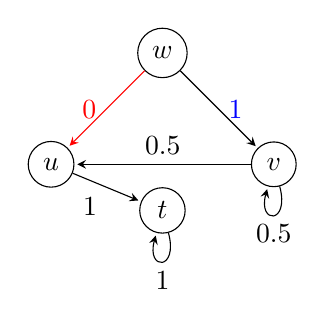
\begin{tikzpicture}[->,>=stealth,shorten >=1pt,auto,node distance=2cm]
        
        % Nodes
        \node[circle,draw] (w) {$w$};
        \node[circle,draw,below left of=w] (u) {$u$};
        \node[circle,draw,below right of=w] (v) {$v$};
        \node[circle,draw,below of=w] (t) {$t$};
        
        % Edges
        \path (w) edge[red] node[left,red] {$0$} (u)
              (w) edge node[right,blue] {$1$} (v)
              (u) edge node[below left] {$1$} (t)
              (v) edge node[above] {$0.5$} (u)
              (v) edge [loop below] node {$0.5$} (v)
              (t) edge [loop below] node {$1$} (t);
        
        \end{tikzpicture}
    \caption{The probabilistic Kripke model $(W,P^{-(w,u)}_{0.4},V)$.}
    \label{fig:sabotage}
\end{figure}
\end{example}

In general we will need to deal with nested updates over the original probability matrix $P$ of a model $\model$. Thus, we need to make sure that such a sequence of updates over $P$ leads to a well-formed probability matrix. We make these aspects precise in the following definition.

\begin{definition}[Sabotage well-formed]
    \label{def:sab-well-found}
    Let $\model=(W,P,V)$ be a probabilistic Kripke model. Let $\bar{\rho}=\rho_1,\dots,\rho_n$ and ${\overline{wv}}=(w_1,v_1),\ldots,(w_n,v_n)$ be two sequences such that $n\geq 0$, and for all $1\leq i \leq n$, $\rho_i\in]0,1]$ and $w_i,v_i\in W$. 
    
    For $0\leq k \leq n$,  $\bar{\rho}_k=\rho_1,\dots,\rho_k$ and ${\overline{wv}}_k=(w_1,v_1),\ldots(w_k,v_k)$ ($k=0$ yields empty sequences, denoted by $\varepsilon$). 
    We also define $\bar{\rho}\cdot \sigma=\rho_1,\dots,\rho_n,\sigma$ and ${\overline{wv}}\cdot(u,t)=(w_1,v_1),\ldots(w_k,v_k),(u,t)$, and define inductively $P^{-\overline{wv}}_{\bar{\rho}}$ as:
    $P_{\varepsilon}^{-\varepsilon}=P$ and $P_{\rho_k\cdot\sigma}^{-\overline{wv}\cdot (u,t)}= (P_{\rho_k}^{-\overline{wv}})^{-(u,t)}_\sigma$.

    Thus, we say that the updated matrix $P^{-\overline{wv}}_{\bar{\rho}}$ is \emph{well-formed (from $P$) for sabotage} if for all $0\leq j < n$, $\rho_{j+1} \leq P^{-{\overline{wv}}_j}_{\bar{\rho}_j}(w_{j+1},v_{j+1})\neq 1$. 
\end{definition}

\subsection{Probabilistic Bridge Operator}

Now it is time to move to the bridge case, generalizing~\cite{Fervari14,ArecesFH15}, and being more specific that in the graded case from~\cite{FFM25}. The idea is that if there no way to access some point with a certain probability value, the evaluation is moved to such a point, and the value is added to the traversed edge. This is similar to the graded case, but here we need to be careful to maintain the probability distribution. This is achieved by proportionally transferring the value from other edges to the intended one.

\begin{definition}
    
The satisfiability relation $\models$ is defined as in Def.~\ref{def:sab-semantics} for the Boolean cases and for $\Diamond_\rho$, and extended with the following case:
\[
    \begin{array}{l@{\ \ }c@{\ \ }l}
    %  \model,w\models p & \iff &  w\in V(p)\\ 
    %  \model,w\models\neg\varphi & \iff & \model,w\not\models\varphi \\         \model,w\models \varphi\vee\psi & \iff & \model,w\models\varphi \text{ or } \model,w\models\psi \\
    % \model,w\models \Diamond_\rho \varphi & \iff &  \displaystyle\sum_{\{v \in W \mid \model,v\models\varphi\}} P(w,v) \geq \rho \\
    \model,w\models \blacklozenge_\rho \varphi & \iff &  \text{exists } v\in W \mbox{ s.t. } \ P(w,v)+\rho\leq 1, \mbox{ and } \model^{+(w,v)}_\rho, v \models\varphi, 
    \end{array}
\]
    % \begin{itemize}
    %     \item$\model,w\models p \mbox{ iff } w\in V(p)$;
    %     \item$\model\operatorname{val}(s, \lnot X) = \text{true} \ \text{iff} \ \operatorname{val}(s, X) = \text{false}$;
    %     \item$\model\operatorname{val}(s, X \land Y) = \text{true} \ \text{iff} \ \operatorname{val}(s, X) = \operatorname{val}(s, Y) = \text{true}$;
    %     \item $\model,w\models \Diamond_\rho \varphi \mbox{ iff } \Sigma_{(v \mid \model,v\models\varphi)} P(w,v) \geq \rho$;
    %      \item$\model,w\models \blacklozenge_\rho \varphi \mbox{ iff } \exists \ u,v\in W \mbox{ s.t. } u\neq v, \ P(w,v)+\rho\leq 1, \mbox{ and } \model^{v+\rho}, v \models\varphi$.
    % \end{itemize}
where $\model^{+(w,v)}_\rho = (W, P^{+(w,v)}_\rho,V)$, with:
\begin{itemize}
    \item $P^{+(w,v)}_\rho(w,v)=P(w,v)+\rho$;
    %\textcolor{blue}{MAM: If $\rho> P(w,v)$?} \textcolor{red}{RF: this condition is taken care in the  precondition of the modality. It depends how we want to define it.MAM: OK}
    \item $P^{+(w,v)}_\rho(w,t)=P(w,t)-
\dfrac{\rho.P(w,t)}{1-P(w,v)}$, if $ t \neq v$;
    \item $P^{+(w,v)}_\rho(s,t)=P(s,t)$, if $s\neq w$.
\end{itemize}

Again, note that $\model^{+(w,v)}_\rho$ is a well-formed model.

In what follows, we will denote  by $\model , u \equiv_b \model' , u'$ whenever $\model , u \models \varphi$ iff $\model' , u' \models \varphi$ for all $\varphi \in \form $ with the bridge semantics.

\end{definition}

The semantics of the bridge operator depicts a case where either the probability of an event to occur increases or some new transition is possible. Thus, the probability assigned to the other edges that also leave from the same origin state must decrease. As in the case of the ``sabotage'', this reduction is obtained in a proportional way, based on the previous value of each edge probability. This is illustrated in Example \ref{ex:brid}.

\begin{example}\label{ex:brid}
Let us recall the model $(W,P,V)$ from Example \ref{ex1} and check if $v$ satisfies $\blacklozenge_{0.4} q$. By the semantics we have 
$\model,v\models\blacklozenge_{0.4} q$ iff $\exists x\in W$ s.t. $0.4\leq \ P(v,x)\neq 1$,  and $\model^{+(v,x)}_{0.4}, x \models q$.

$P(v,x)\leq 0.4$ implies $x=w$ or $x=t$. Although $w\not\in V(p)$, the formula is satisfied because $\model^{+(v,t)}_{0.4}, t \models p$. Moreover, the model $\model^{+(v,t)}_{0.4}=(W,P^{+(v,t)}_{0.4},V)$ is illustrated in Fig. \ref{fig:bridge}.

\begin{figure}[!ht]
    \centering
        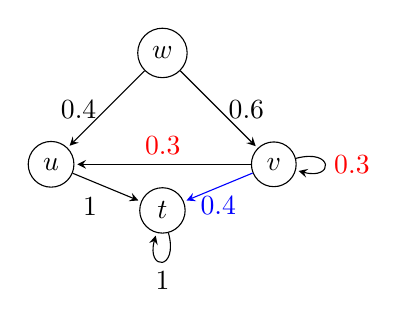
\begin{tikzpicture}[->,>=stealth,shorten >=1pt,auto,node distance=2cm]
        
        % Nodes
        \node[circle,draw] (w) {$w$};
        \node[circle,draw,below left of=w] (u) {$u$};
        \node[circle,draw,below right of=w] (v) {$v$};
        \node[circle,draw,below of=w] (t) {$t$};
        
        % Edges
        \path (w) edge node[left] {$0.4$} (u)
              (w) edge node[right] {$0.6$} (v)
              (u) edge node[below left] {$1$} (t)
              (v) edge node[above,red] {$0.3$} (u)
              (v) edge [loop right] node[red] {$0.3$} (v)
              (v) edge [below,blue] node[blue] {$0.4$} (t)
              (t) edge [loop below] node {$1$} (t);
        
        \end{tikzpicture}
    \caption{The probabilistic Kripke model $(W,P^{+(v,t)}_{0.4},V)$.}
    \label{fig:bridge}
\end{figure}
\end{example}

Again, we need to establish when a sequence of updates is well-formed.

\begin{definition}[Bridge well-formed]
    \label{def:bridge-well-found}
    Let $\model=(W,P,V)$, $\bar{\rho}=\rho_1,\dots,\rho_n$ and ${\overline{wv}}=(w_1,v_1),\ldots,(w_n,v_n)$ as in Def.~\ref{def:sab-well-found}. Let $P^{+\overline{wv}}_{\bar{\rho}}$
    be defined analogously to~$P^{-\overline{wv}}_{\bar{\rho}}$. 
    % For $0\leq k \leq n$,  $\bar{\rho}_k=\rho_1,\dots,\rho_k$ and ${\overline{wv}}_k=(w_1,v_1),\ldots(w_k,v_k)$ ($k=0$ yields empty sequences $\varepsilon$). 
    % We also define $\bar{\rho}\cdot \sigma=\rho_1,\dots,\rho_n,\sigma$ and ${\overline{wv}}\cdot(u,t)=(w_1,v_1),\ldots(w_k,v_k),(u,t)$, and define inductively $P^{-\overline{wv}}_{\bar{\rho}}$ as:
    % $P_{\varepsilon}^{-\varepsilon}=P$ and $P_{\rho_k\cdot\sigma}^{-\overline{wv}\cdot (u,t)}= (P_{\rho_k}^{-\overline{wv}})^{-(u,t)}_\sigma$.

    We say that the updated matrix $P^{+\overline{wv}}_{\bar{\rho}}$ is \emph{well-formed (from $P$) for bridge} if for all $0\leq j < n$, $ P^{+{\overline{wv}}_j}_{\bar{\rho}_j}(w_{j+1},v_{j+1}) + \rho_{j+1}\leq 1$. 
\end{definition}

\subsection{Probabilistic Swap Operator}

We conclude this section by introducing a local swap modality, inspired by~\cite{ArecesFH14}. In a non-probabilistic setting, a swap modality can be seen as a double operation in which we remove an edge $(w,v)$ and we add its converse edge $(v,w)$. We can mimic this behaviour here, by taking both the precautions as in the sabotage and bridge: once some value $\rho$ is decreased between a node $w$ and $v$, we need to make sure that such a value is reassigned to the rest of successors of $w$. But also, since the value $\rho$ is increased from $v$ to $w$, now we need to remove such a value from $v$-successors proportionally. We formalize this idea in the semantics definition below.

\begin{definition}
    \label{def:swap-semantics}
    The satisfiability relation $\models$ is defined as in Def.~\ref{def:sab-semantics} for the Boolean cases and for $\Diamond_\rho$, and extended with the following case:
\[
    \begin{array}{l@{\ \ }c@{\ \ }l}
    %  \model,w\models p & \iff &  w\in V(p)\\ 
    %  \model,w\models\neg\varphi & \iff & \model,w\not\models\varphi \\         \model,w\models \varphi\vee\psi & \iff & \model,w\models\varphi \text{ or } \model,w\models\psi \\
    % \model,w\models \Diamond_\rho \varphi & \iff &  \displaystyle\sum_{\{v \in W \mid \model,v\models\varphi\}} P(w,v) \geq \rho \\
    \model,w\models \blacklozenge_\rho \varphi & \iff & \text{there exists }v\in W\text{ s.t. } \\
    && \rho \leq P(w,v)\neq 1,\quad P(v,w)+\rho\leq 1 \text{ and }\model^{*(w,v)}_\rho, v \models\varphi,
    \end{array}
\]
    % \begin{itemize}
    %     \item$\model,w\models p \mbox{ iff } w\in V(p)$;
    %     \item$\model\operatorname{val}(s, \lnot X) = \text{true} \ \text{iff} \ \operatorname{val}(s, X) = \text{false}$;
    %     \item$\model\operatorname{val}(s, X \land Y) = \text{true} \ \text{iff} \ \operatorname{val}(s, X) = \operatorname{val}(s, Y) = \text{true}$;
    %     \item $\model,w\models \Diamond_\rho \varphi \mbox{ iff } \Sigma_{(v \mid \model,v\models\varphi)} P(w,v) \geq \rho$;
    %      \item$\model,w\models \blacklozenge_\rho \varphi \mbox{ iff } \exists \ u,v\in W \mbox{ s.t. } u\neq v, \ P(w,v)+\rho\leq 1, \mbox{ and } \model^{v+\rho}, v \models\varphi$.
    % \end{itemize}
where $\model^{*(w,v)}_\rho = (W, P^{*(w,v)}_\rho,V)$, with:
\begin{itemize}
    \item $P^{*(w,v)}_\rho(w,v)=P(w,v)-\rho$;
    \item $P^{*(w,v)}_\rho(v,w)=P(v,w)+\rho$;
    \item $P^{*(w,v)}_\rho(w,t)=P(w,t)+
\dfrac{\rho.P(w,t)}{1-P(w,v)}$, if $ t \neq v$;
    \item $P^{*(w,v)}_\rho(v,t)=P(v,t)-
\dfrac{\rho.P(v,t)}{1-P(v,w)}$, if $ t \neq w$;
    \item $P^{*(w,v)}_\rho(s,t)=P(s,t)$, if $v\neq s\neq w$.
\end{itemize}

Again, note that $\model^{*(w,v)}_\rho$ is a well-formed model.

In what follows, we will denote  by $\model , u \equiv_w \model' , u'$ whenever $\model , u \models \varphi$ iff $\model' , u' \models \varphi$ for all $\varphi \in \form $ with the swap semantics.

\end{definition}

Again, we need to establish when a sequence of updates is well-formed.

\begin{definition}[Swap well-formed]
    \label{def:swap-well-found}
    Let $\model=(W,P,V)$, $\bar{\rho}=\rho_1,\dots,\rho_n$ and ${\overline{wv}}=(w_1,v_1),\ldots,(w_n,v_n)$ as in Def.~\ref{def:sab-well-found}. Let $P^{*\overline{wv}}_{\bar{\rho}}$
    be defined analogously to~$P^{-\overline{wv}}_{\bar{\rho}}$. 
    % For $0\leq k \leq n$,  $\bar{\rho}_k=\rho_1,\dots,\rho_k$ and ${\overline{wv}}_k=(w_1,v_1),\ldots(w_k,v_k)$ ($k=0$ yields empty sequences $\varepsilon$). 
    % We also define $\bar{\rho}\cdot \sigma=\rho_1,\dots,\rho_n,\sigma$ and ${\overline{wv}}\cdot(u,t)=(w_1,v_1),\ldots(w_k,v_k),(u,t)$, and define inductively $P^{-\overline{wv}}_{\bar{\rho}}$ as:
    % $P_{\varepsilon}^{-\varepsilon}=P$ and $P_{\rho_k\cdot\sigma}^{-\overline{wv}\cdot (u,t)}= (P_{\rho_k}^{-\overline{wv}})^{-(u,t)}_\sigma$.

    We say that the updated matrix $P^{*\overline{wv}}_{\bar{\rho}}$ is \emph{well-formed (from $P$) for swap} if for all $0\leq j < n$, $\rho_{j+1}\leq P^{*{\overline{wv}}_j}_{\bar{\rho}_j}(w_{j+1},v_{j+1})\neq 1$ and $P^{*{\overline{wv}}_j}_{\bar{\rho}_j}(v_{j+1},w_{j+1})+\rho_{j+1}\leq 1$. 
\end{definition}